\documentclass[a4paper]{book}
\usepackage{makeidx}
\usepackage{graphicx}
\usepackage{multicol}
\usepackage{float}
\usepackage{listings}
\usepackage{color}
\usepackage{ifthen}
\usepackage[table]{xcolor}
\usepackage{textcomp}
\usepackage{alltt}
\usepackage{ifpdf}
\ifpdf
\usepackage[pdftex,
            pagebackref=true,
            colorlinks=true,
            linkcolor=blue,
            unicode
           ]{hyperref}
\else
\usepackage[ps2pdf,
            pagebackref=true,
            colorlinks=true,
            linkcolor=blue,
            unicode
           ]{hyperref}
\usepackage{pspicture}
\fi
\usepackage[utf8]{inputenc}
\usepackage{mathptmx}
\usepackage[scaled=.90]{helvet}
\usepackage{courier}
\usepackage{doxygen}
\lstset{language=C++,inputencoding=utf8,basicstyle=\footnotesize,breaklines=true,breakatwhitespace=true,tabsize=8,numbers=left }
\makeindex
\setcounter{tocdepth}{3}
\renewcommand{\footrulewidth}{0.4pt}
\begin{document}
\hypersetup{pageanchor=false}
\begin{titlepage}
\vspace*{7cm}
\begin{center}
{\Large Reference Manual}\\
\vspace*{1cm}
{\large Generated by Doxygen 1.7.3}\\
\vspace*{0.5cm}
{\small Sat Apr 2 2011 13:06:35}\\
\end{center}
\end{titlepage}
\clearemptydoublepage
\pagenumbering{roman}
\tableofcontents
\clearemptydoublepage
\pagenumbering{arabic}
\hypersetup{pageanchor=true}
\chapter{Class Index}
\section{Class List}
Here are the classes, structs, unions and interfaces with brief descriptions:\begin{DoxyCompactList}
\item\contentsline{section}{\hyperlink{struct_t_a_b_l_e}{TABLE} }{\pageref{struct_t_a_b_l_e}}{}
\end{DoxyCompactList}

\chapter{File Index}
\section{File List}
Here is a list of all files with brief descriptions:\begin{DoxyCompactList}
\item\contentsline{section}{\hyperlink{_bradshaw-_mansfield-_assn2-_h_a_s_h_prog_8cpp}{Bradshaw-\/Mansfield-\/Assn2-\/HASHProg.cpp} }{\pageref{_bradshaw-_mansfield-_assn2-_h_a_s_h_prog_8cpp}}{}
\end{DoxyCompactList}

\chapter{Class Documentation}
\hypertarget{struct_t_a_b_l_e}{
\section{TABLE Struct Reference}
\label{struct_t_a_b_l_e}\index{TABLE@{TABLE}}
}


Collaboration diagram for TABLE:\nopagebreak
\begin{figure}[H]
\begin{center}
\leavevmode
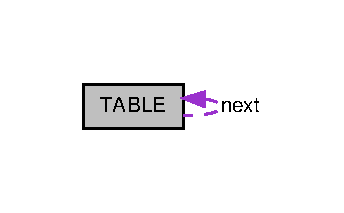
\includegraphics[width=165pt]{struct_t_a_b_l_e__coll__graph}
\end{center}
\end{figure}
\subsection*{Public Member Functions}
\begin{DoxyCompactItemize}
\item 
\hyperlink{struct_t_a_b_l_e_a34ca35df0c02a42a2667b918ac8949b9}{TABLE} ()
\end{DoxyCompactItemize}
\subsection*{Public Attributes}
\begin{DoxyCompactItemize}
\item 
int \hyperlink{struct_t_a_b_l_e_aca8b660b95cd57c4ac1985b870651ce6}{key}
\item 
\hyperlink{struct_t_a_b_l_e}{TABLE} $\ast$ \hyperlink{struct_t_a_b_l_e_a9a6386994116363347f6a485410c4f02}{next}
\end{DoxyCompactItemize}


\subsection{Detailed Description}


Definition at line 44 of file Bradshaw-\/Mansfield-\/Assn2-\/DLLProg.cpp.



\subsection{Constructor \& Destructor Documentation}
\hypertarget{struct_t_a_b_l_e_a34ca35df0c02a42a2667b918ac8949b9}{
\index{TABLE@{TABLE}!TABLE@{TABLE}}
\index{TABLE@{TABLE}!TABLE@{TABLE}}
\subsubsection[{TABLE}]{\setlength{\rightskip}{0pt plus 5cm}TABLE::TABLE (
\begin{DoxyParamCaption}
{}
\end{DoxyParamCaption}
)\hspace{0.3cm}{\ttfamily  \mbox{[}inline\mbox{]}}}}
\label{struct_t_a_b_l_e_a34ca35df0c02a42a2667b918ac8949b9}


Definition at line 45 of file Bradshaw-\/Mansfield-\/Assn2-\/DLLProg.cpp.



\subsection{Member Data Documentation}
\hypertarget{struct_t_a_b_l_e_aca8b660b95cd57c4ac1985b870651ce6}{
\index{TABLE@{TABLE}!key@{key}}
\index{key@{key}!TABLE@{TABLE}}
\subsubsection[{key}]{\setlength{\rightskip}{0pt plus 5cm}int {\bf TABLE::key}}}
\label{struct_t_a_b_l_e_aca8b660b95cd57c4ac1985b870651ce6}


Definition at line 46 of file Bradshaw-\/Mansfield-\/Assn2-\/DLLProg.cpp.

\hypertarget{struct_t_a_b_l_e_a9a6386994116363347f6a485410c4f02}{
\index{TABLE@{TABLE}!next@{next}}
\index{next@{next}!TABLE@{TABLE}}
\subsubsection[{next}]{\setlength{\rightskip}{0pt plus 5cm}{\bf TABLE} $\ast$ {\bf TABLE::next}}}
\label{struct_t_a_b_l_e_a9a6386994116363347f6a485410c4f02}


Definition at line 47 of file Bradshaw-\/Mansfield-\/Assn2-\/DLLProg.cpp.



The documentation for this struct was generated from the following files:\begin{DoxyCompactItemize}
\item 
\hyperlink{_bradshaw-_mansfield-_assn2-_d_l_l_prog_8cpp}{Bradshaw-\/Mansfield-\/Assn2-\/DLLProg.cpp}\item 
\hyperlink{hash_t_a_b_l_e_8cpp}{hashTABLE.cpp}\end{DoxyCompactItemize}

\chapter{File Documentation}
\hypertarget{_bradshaw-_mansfield-_assn2-_h_a_s_h_prog_8cpp}{
\section{Bradshaw-\/Mansfield-\/Assn2-\/HASHProg.cpp File Reference}
\label{_bradshaw-_mansfield-_assn2-_h_a_s_h_prog_8cpp}\index{Bradshaw-\/Mansfield-\/Assn2-\/HASHProg.cpp@{Bradshaw-\/Mansfield-\/Assn2-\/HASHProg.cpp}}
}
{\ttfamily \#include $<$iostream$>$}\par
{\ttfamily \#include $<$iomanip$>$}\par
{\ttfamily \#include $<$string$>$}\par
{\ttfamily \#include $<$cstdlib$>$}\par
{\ttfamily \#include $<$cmath$>$}\par
{\ttfamily \#include $<$cstddef$>$}\par
Include dependency graph for Bradshaw-\/Mansfield-\/Assn2-\/HASHProg.cpp:\nopagebreak
\begin{figure}[H]
\begin{center}
\leavevmode
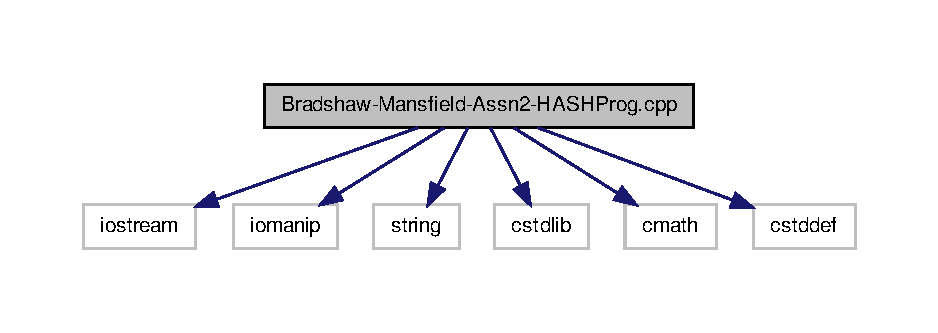
\includegraphics[width=400pt]{_bradshaw-_mansfield-_assn2-_h_a_s_h_prog_8cpp__incl}
\end{center}
\end{figure}
\subsection*{Classes}
\begin{DoxyCompactItemize}
\item 
struct \hyperlink{struct_t_a_b_l_e}{TABLE}
\end{DoxyCompactItemize}
\subsection*{Functions}
\begin{DoxyCompactItemize}
\item 
void \hyperlink{_bradshaw-_mansfield-_assn2-_h_a_s_h_prog_8cpp_ad0ff1b56e8aa2267183dc975be2704c3}{HeaderMain} ()
\item 
int \hyperlink{_bradshaw-_mansfield-_assn2-_h_a_s_h_prog_8cpp_ad02a3d3bea24e6a374d52753e741ae54}{RandNums} (int $\ast$)
\item 
int \hyperlink{_bradshaw-_mansfield-_assn2-_h_a_s_h_prog_8cpp_a0ab6301502b50757d27084788bab0db3}{HashTableSize} ()
\item 
int \hyperlink{_bradshaw-_mansfield-_assn2-_h_a_s_h_prog_8cpp_a3cbbd19bf1195623cc2c00ce8b55eaeb}{hash} (int, int)
\item 
void \hyperlink{_bradshaw-_mansfield-_assn2-_h_a_s_h_prog_8cpp_ac4885dc21b261220f2a030b1ad06aec5}{ThreeHashMethods} ()
\item 
int $\ast$ \hyperlink{_bradshaw-_mansfield-_assn2-_h_a_s_h_prog_8cpp_aa4c8e3922c8cd75082eae40ba8cd0205}{OA\_\-LinearProbe} (int $\ast$, int, int\mbox{[}$\,$\mbox{]})
\item 
void \hyperlink{_bradshaw-_mansfield-_assn2-_h_a_s_h_prog_8cpp_aa08a3d5e09643b1011e506d60a89a7f2}{OA\_\-DoubleHash} (int $\ast$, int, int\mbox{[}$\,$\mbox{]}, bool \&)
\item 
void \hyperlink{_bradshaw-_mansfield-_assn2-_h_a_s_h_prog_8cpp_ad730cee6dc4ea13d5fabcec47b736c79}{SeparateChaining} (int $\ast$, int, \hyperlink{struct_t_a_b_l_e}{TABLE}\mbox{[}$\,$\mbox{]})
\item 
int \hyperlink{_bradshaw-_mansfield-_assn2-_h_a_s_h_prog_8cpp_acb3d9aabc9ab7fbb9d3ae15ad62c32f1}{HashDriver} (int, int\mbox{[}$\,$\mbox{]}, double)
\item 
void \hyperlink{_bradshaw-_mansfield-_assn2-_h_a_s_h_prog_8cpp_a74bb3e2823ba913f28e3f6711e045824}{LinearProbe} (int \&, int\mbox{[}$\,$\mbox{]}, int, int, int \&)
\item 
int \hyperlink{_bradshaw-_mansfield-_assn2-_h_a_s_h_prog_8cpp_a7b947e56197fe93937e40b0c987f40fb}{DoubleHash} (int, int, int)
\item 
int \hyperlink{_bradshaw-_mansfield-_assn2-_h_a_s_h_prog_8cpp_a1cfe5833c4e03ff0473ca3e3b87f9f1d}{TableOneMatch} (int $\ast$, int $\ast$, int, int, int)
\item 
int \hyperlink{_bradshaw-_mansfield-_assn2-_h_a_s_h_prog_8cpp_ab7be41246bbc3491cbe4151458a15f39}{TableTwoMatch} (int $\ast$, \hyperlink{struct_t_a_b_l_e}{TABLE}\mbox{[}$\,$\mbox{]}, int, int)
\item 
void \hyperlink{_bradshaw-_mansfield-_assn2-_h_a_s_h_prog_8cpp_ac833bf25caea2f934fd8d75e2986997c}{DisplayResults} (int, double, int)
\item 
int \hyperlink{_bradshaw-_mansfield-_assn2-_h_a_s_h_prog_8cpp_ae66f6b31b5ad750f1fe042a706a4e3d4}{main} ()
\item 
int \hyperlink{_bradshaw-_mansfield-_assn2-_h_a_s_h_prog_8cpp_ae9957e8e2a204d621e9f9cc2999adf56}{Hash} (int key, int listSize)
\item 
int \hyperlink{_bradshaw-_mansfield-_assn2-_h_a_s_h_prog_8cpp_aba56e572dc851c7863847efa4a3a1f22}{DoubleHash} (int key, int listSize)
\item 
int $\ast$ \hyperlink{_bradshaw-_mansfield-_assn2-_h_a_s_h_prog_8cpp_aa342d426f7a6fa643a100ba04bc8e46e}{OA\_\-LinearProbe} (int $\ast$randArray, int tbSize, int $\ast$hashTable)
\end{DoxyCompactItemize}
\subsection*{Variables}
\begin{DoxyCompactItemize}
\item 
const int \hyperlink{_bradshaw-_mansfield-_assn2-_h_a_s_h_prog_8cpp_a80697a51c12117a5eae4ada58d27e1c2}{MAX\_\-INT\_\-SIZE} = 30000
\item 
const int \hyperlink{_bradshaw-_mansfield-_assn2-_h_a_s_h_prog_8cpp_a2e30ee6cd6a71066a4c99da7204c73bd}{MIN\_\-INT\_\-SIZE} = 1
\item 
const int \hyperlink{_bradshaw-_mansfield-_assn2-_h_a_s_h_prog_8cpp_ac3e309d0e80c3dd569ed3cfb701075a8}{NUM\_\-PROBING\_\-LOOPS} = 3
\item 
const int \hyperlink{_bradshaw-_mansfield-_assn2-_h_a_s_h_prog_8cpp_a92e00f871716652e494af2741a4794bd}{MIN\_\-HASH\_\-TABLE\_\-SIZE} = 6500
\item 
const int \hyperlink{_bradshaw-_mansfield-_assn2-_h_a_s_h_prog_8cpp_ad2624222b2a41e40f795baff70c1d20c}{MAX\_\-KEYS} = 5000
\item 
const int \hyperlink{_bradshaw-_mansfield-_assn2-_h_a_s_h_prog_8cpp_a02ce5f32cab205c8455bd8b976085c50}{NUM\_\-ITEMS\_\-TO\_\-SEARCH} = 2500
\item 
const double \hyperlink{_bradshaw-_mansfield-_assn2-_h_a_s_h_prog_8cpp_ad619de5a53a38d732b9c5da01523a23e}{NUM\_\-ITEMS\_\-TO\_\-SEARCH\_\-DBL} = 2500.00
\item 
const double \hyperlink{_bradshaw-_mansfield-_assn2-_h_a_s_h_prog_8cpp_a3a0ca86f28ff2c4d31143f5f3d6ca40a}{MAX\_\-KEYS\_\-DBL} = 5000.00
\end{DoxyCompactItemize}


\subsection{Function Documentation}
\hypertarget{_bradshaw-_mansfield-_assn2-_h_a_s_h_prog_8cpp_ac833bf25caea2f934fd8d75e2986997c}{
\index{Bradshaw-\/Mansfield-\/Assn2-\/HASHProg.cpp@{Bradshaw-\/Mansfield-\/Assn2-\/HASHProg.cpp}!DisplayResults@{DisplayResults}}
\index{DisplayResults@{DisplayResults}!Bradshaw-Mansfield-Assn2-HASHProg.cpp@{Bradshaw-\/Mansfield-\/Assn2-\/HASHProg.cpp}}
\subsubsection[{DisplayResults}]{\setlength{\rightskip}{0pt plus 5cm}void DisplayResults (
\begin{DoxyParamCaption}
\item[{int}]{colCount, }
\item[{double}]{loadFactor, }
\item[{int}]{loop}
\end{DoxyParamCaption}
)}}
\label{_bradshaw-_mansfield-_assn2-_h_a_s_h_prog_8cpp_ac833bf25caea2f934fd8d75e2986997c}
FUNCTION: DisplayResults DESCRIPTION: Calculates Knuth results per collision type. Displays actual results vs Knuth predicted results INPUT: Parameters: colCount: The count of how many searches were performed. loadFactor: The calculated load factor loop: The loop number to set the display per collision type. IMPLEMENTED BY: Jeremy Bradshaw 

Definition at line 448 of file Bradshaw-\/Mansfield-\/Assn2-\/HASHProg.cpp.



Here is the caller graph for this function:\nopagebreak
\begin{figure}[H]
\begin{center}
\leavevmode
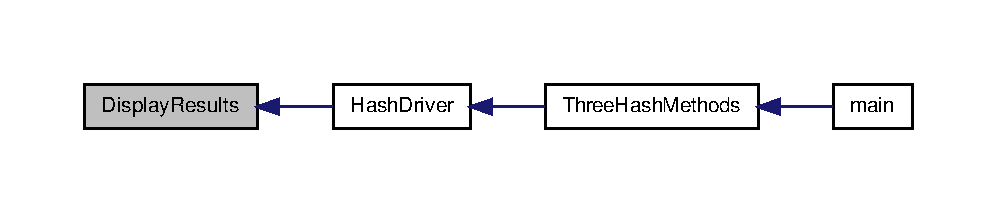
\includegraphics[width=400pt]{_bradshaw-_mansfield-_assn2-_h_a_s_h_prog_8cpp_ac833bf25caea2f934fd8d75e2986997c_icgraph}
\end{center}
\end{figure}


\hypertarget{_bradshaw-_mansfield-_assn2-_h_a_s_h_prog_8cpp_aba56e572dc851c7863847efa4a3a1f22}{
\index{Bradshaw-\/Mansfield-\/Assn2-\/HASHProg.cpp@{Bradshaw-\/Mansfield-\/Assn2-\/HASHProg.cpp}!DoubleHash@{DoubleHash}}
\index{DoubleHash@{DoubleHash}!Bradshaw-Mansfield-Assn2-HASHProg.cpp@{Bradshaw-\/Mansfield-\/Assn2-\/HASHProg.cpp}}
\subsubsection[{DoubleHash}]{\setlength{\rightskip}{0pt plus 5cm}int DoubleHash (
\begin{DoxyParamCaption}
\item[{int}]{key, }
\item[{int}]{listSize}
\end{DoxyParamCaption}
)}}
\label{_bradshaw-_mansfield-_assn2-_h_a_s_h_prog_8cpp_aba56e572dc851c7863847efa4a3a1f22}
FUNCTION: \hyperlink{_bradshaw-_mansfield-_assn2-_h_a_s_h_prog_8cpp_a7b947e56197fe93937e40b0c987f40fb}{DoubleHash()} DESCRIPTION: Performs another modulus hashing algorithm. INPUT: Parameters: key: The number slot for hashing listSize: The user selected list size search: The value to search for OUTPUT: Return Val: key: Returns address found with matching search IMPLEMENTED BY: Jeremy Bradshaw 

Definition at line 150 of file Bradshaw-\/Mansfield-\/Assn2-\/HASHProg.cpp.

\hypertarget{_bradshaw-_mansfield-_assn2-_h_a_s_h_prog_8cpp_a7b947e56197fe93937e40b0c987f40fb}{
\index{Bradshaw-\/Mansfield-\/Assn2-\/HASHProg.cpp@{Bradshaw-\/Mansfield-\/Assn2-\/HASHProg.cpp}!DoubleHash@{DoubleHash}}
\index{DoubleHash@{DoubleHash}!Bradshaw-Mansfield-Assn2-HASHProg.cpp@{Bradshaw-\/Mansfield-\/Assn2-\/HASHProg.cpp}}
\subsubsection[{DoubleHash}]{\setlength{\rightskip}{0pt plus 5cm}int DoubleHash (
\begin{DoxyParamCaption}
\item[{int}]{, }
\item[{int}]{, }
\item[{int}]{}
\end{DoxyParamCaption}
)}}
\label{_bradshaw-_mansfield-_assn2-_h_a_s_h_prog_8cpp_a7b947e56197fe93937e40b0c987f40fb}


Here is the caller graph for this function:\nopagebreak
\begin{figure}[H]
\begin{center}
\leavevmode
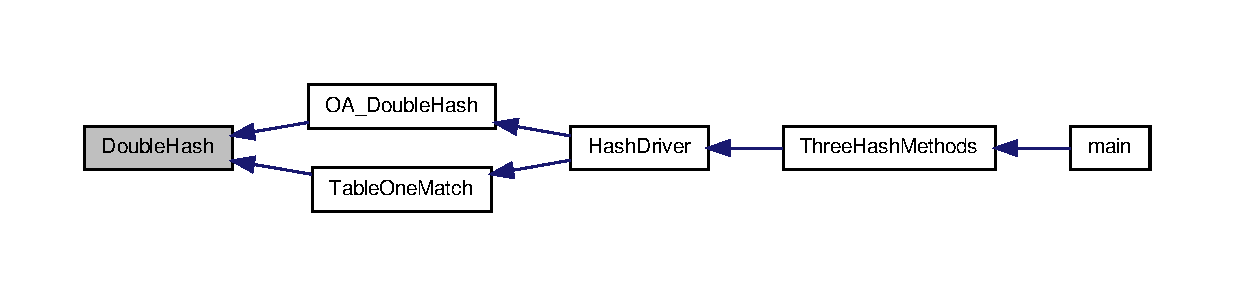
\includegraphics[width=400pt]{_bradshaw-_mansfield-_assn2-_h_a_s_h_prog_8cpp_a7b947e56197fe93937e40b0c987f40fb_icgraph}
\end{center}
\end{figure}


\hypertarget{_bradshaw-_mansfield-_assn2-_h_a_s_h_prog_8cpp_a3cbbd19bf1195623cc2c00ce8b55eaeb}{
\index{Bradshaw-\/Mansfield-\/Assn2-\/HASHProg.cpp@{Bradshaw-\/Mansfield-\/Assn2-\/HASHProg.cpp}!hash@{hash}}
\index{hash@{hash}!Bradshaw-Mansfield-Assn2-HASHProg.cpp@{Bradshaw-\/Mansfield-\/Assn2-\/HASHProg.cpp}}
\subsubsection[{hash}]{\setlength{\rightskip}{0pt plus 5cm}int hash (
\begin{DoxyParamCaption}
\item[{int}]{, }
\item[{int}]{}
\end{DoxyParamCaption}
)}}
\label{_bradshaw-_mansfield-_assn2-_h_a_s_h_prog_8cpp_a3cbbd19bf1195623cc2c00ce8b55eaeb}
\hypertarget{_bradshaw-_mansfield-_assn2-_h_a_s_h_prog_8cpp_ae9957e8e2a204d621e9f9cc2999adf56}{
\index{Bradshaw-\/Mansfield-\/Assn2-\/HASHProg.cpp@{Bradshaw-\/Mansfield-\/Assn2-\/HASHProg.cpp}!Hash@{Hash}}
\index{Hash@{Hash}!Bradshaw-Mansfield-Assn2-HASHProg.cpp@{Bradshaw-\/Mansfield-\/Assn2-\/HASHProg.cpp}}
\subsubsection[{Hash}]{\setlength{\rightskip}{0pt plus 5cm}int Hash (
\begin{DoxyParamCaption}
\item[{int}]{key, }
\item[{int}]{listSize}
\end{DoxyParamCaption}
)}}
\label{_bradshaw-_mansfield-_assn2-_h_a_s_h_prog_8cpp_ae9957e8e2a204d621e9f9cc2999adf56}
FUNCTION: \hyperlink{_bradshaw-_mansfield-_assn2-_h_a_s_h_prog_8cpp_ae9957e8e2a204d621e9f9cc2999adf56}{Hash()} DESCRIPTION: Basic modulus hashing algorithm. INPUT: Parameters: key: The number slot for hashing listSize: The user selected list size OUTPUT: Return Val: address: Hashed address IMPLEMENTED BY: Jason Mansfield 

Definition at line 131 of file Bradshaw-\/Mansfield-\/Assn2-\/HASHProg.cpp.



Here is the caller graph for this function:\nopagebreak
\begin{figure}[H]
\begin{center}
\leavevmode
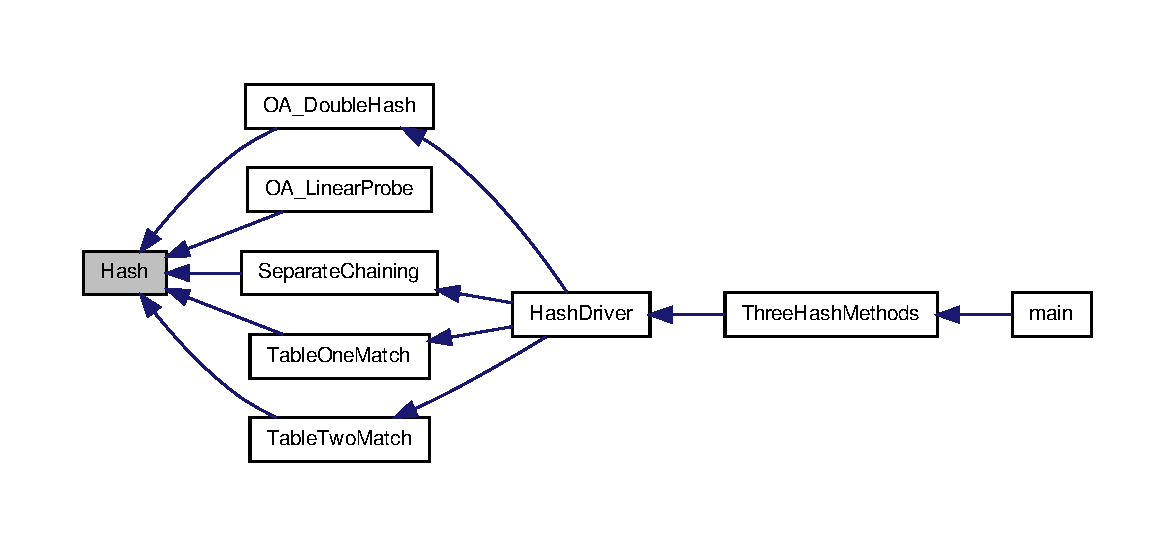
\includegraphics[width=400pt]{_bradshaw-_mansfield-_assn2-_h_a_s_h_prog_8cpp_ae9957e8e2a204d621e9f9cc2999adf56_icgraph}
\end{center}
\end{figure}


\hypertarget{_bradshaw-_mansfield-_assn2-_h_a_s_h_prog_8cpp_acb3d9aabc9ab7fbb9d3ae15ad62c32f1}{
\index{Bradshaw-\/Mansfield-\/Assn2-\/HASHProg.cpp@{Bradshaw-\/Mansfield-\/Assn2-\/HASHProg.cpp}!HashDriver@{HashDriver}}
\index{HashDriver@{HashDriver}!Bradshaw-Mansfield-Assn2-HASHProg.cpp@{Bradshaw-\/Mansfield-\/Assn2-\/HASHProg.cpp}}
\subsubsection[{HashDriver}]{\setlength{\rightskip}{0pt plus 5cm}int HashDriver (
\begin{DoxyParamCaption}
\item[{int}]{tbSize, }
\item[{int}]{randArray\mbox{[}$\,$\mbox{]}, }
\item[{double}]{loadFactor}
\end{DoxyParamCaption}
)}}
\label{_bradshaw-_mansfield-_assn2-_h_a_s_h_prog_8cpp_acb3d9aabc9ab7fbb9d3ae15ad62c32f1}
FUNCTION: HashDriver DESCRIPTION: Driver function that calls to the functions used to create the hash table, the collision search functions, and the function that displays the results. Function loops 3 times once for each type. INPUT: Parameters: tbSize: Size requested for hash table. randArray: The random array of MAX\_\-KEYS size ints used for data in all hash tables created. loadFactor: The load factor CALLS TO: \hyperlink{_bradshaw-_mansfield-_assn2-_h_a_s_h_prog_8cpp_aa4c8e3922c8cd75082eae40ba8cd0205}{OA\_\-LinearProbe()} \hyperlink{_bradshaw-_mansfield-_assn2-_h_a_s_h_prog_8cpp_a1cfe5833c4e03ff0473ca3e3b87f9f1d}{TableOneMatch()} \hyperlink{_bradshaw-_mansfield-_assn2-_h_a_s_h_prog_8cpp_ac833bf25caea2f934fd8d75e2986997c}{DisplayResults()} \hyperlink{_bradshaw-_mansfield-_assn2-_h_a_s_h_prog_8cpp_aa08a3d5e09643b1011e506d60a89a7f2}{OA\_\-DoubleHash()} \hyperlink{_bradshaw-_mansfield-_assn2-_h_a_s_h_prog_8cpp_ad730cee6dc4ea13d5fabcec47b736c79}{SeparateChaining()} \hyperlink{_bradshaw-_mansfield-_assn2-_h_a_s_h_prog_8cpp_ab7be41246bbc3491cbe4151458a15f39}{TableTwoMatch()} IMPLEMENTED BY: Jason Mansfield 

Definition at line 288 of file Bradshaw-\/Mansfield-\/Assn2-\/HASHProg.cpp.



Here is the call graph for this function:\nopagebreak
\begin{figure}[H]
\begin{center}
\leavevmode
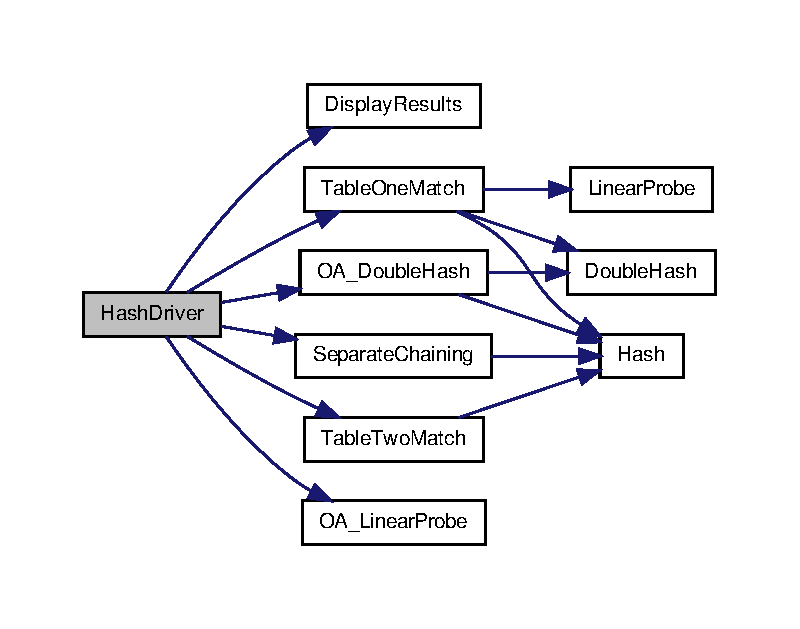
\includegraphics[width=384pt]{_bradshaw-_mansfield-_assn2-_h_a_s_h_prog_8cpp_acb3d9aabc9ab7fbb9d3ae15ad62c32f1_cgraph}
\end{center}
\end{figure}




Here is the caller graph for this function:\nopagebreak
\begin{figure}[H]
\begin{center}
\leavevmode
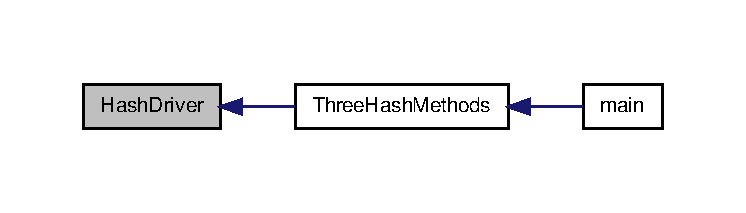
\includegraphics[width=358pt]{_bradshaw-_mansfield-_assn2-_h_a_s_h_prog_8cpp_acb3d9aabc9ab7fbb9d3ae15ad62c32f1_icgraph}
\end{center}
\end{figure}


\hypertarget{_bradshaw-_mansfield-_assn2-_h_a_s_h_prog_8cpp_a0ab6301502b50757d27084788bab0db3}{
\index{Bradshaw-\/Mansfield-\/Assn2-\/HASHProg.cpp@{Bradshaw-\/Mansfield-\/Assn2-\/HASHProg.cpp}!HashTableSize@{HashTableSize}}
\index{HashTableSize@{HashTableSize}!Bradshaw-Mansfield-Assn2-HASHProg.cpp@{Bradshaw-\/Mansfield-\/Assn2-\/HASHProg.cpp}}
\subsubsection[{HashTableSize}]{\setlength{\rightskip}{0pt plus 5cm}int HashTableSize (
\begin{DoxyParamCaption}
{}
\end{DoxyParamCaption}
)}}
\label{_bradshaw-_mansfield-_assn2-_h_a_s_h_prog_8cpp_a0ab6301502b50757d27084788bab0db3}
FUNCTION: \hyperlink{_bradshaw-_mansfield-_assn2-_h_a_s_h_prog_8cpp_a0ab6301502b50757d27084788bab0db3}{HashTableSize()} DESCRIPTION: Requests users desired size Hash Table and returns int OUTPUT: Return Val: userChoose: Int value of user requested hash table size. IMPLEMENTED BY: Jason Mansfield 

Definition at line 205 of file Bradshaw-\/Mansfield-\/Assn2-\/HASHProg.cpp.



Here is the caller graph for this function:\nopagebreak
\begin{figure}[H]
\begin{center}
\leavevmode
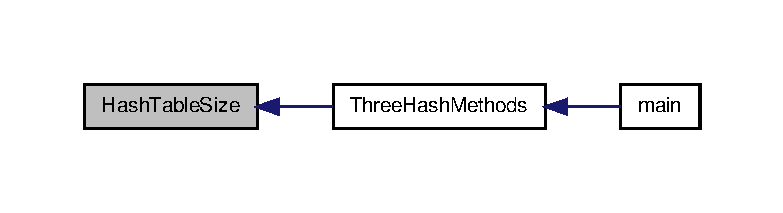
\includegraphics[width=376pt]{_bradshaw-_mansfield-_assn2-_h_a_s_h_prog_8cpp_a0ab6301502b50757d27084788bab0db3_icgraph}
\end{center}
\end{figure}


\hypertarget{_bradshaw-_mansfield-_assn2-_h_a_s_h_prog_8cpp_ad0ff1b56e8aa2267183dc975be2704c3}{
\index{Bradshaw-\/Mansfield-\/Assn2-\/HASHProg.cpp@{Bradshaw-\/Mansfield-\/Assn2-\/HASHProg.cpp}!HeaderMain@{HeaderMain}}
\index{HeaderMain@{HeaderMain}!Bradshaw-Mansfield-Assn2-HASHProg.cpp@{Bradshaw-\/Mansfield-\/Assn2-\/HASHProg.cpp}}
\subsubsection[{HeaderMain}]{\setlength{\rightskip}{0pt plus 5cm}void HeaderMain (
\begin{DoxyParamCaption}
{}
\end{DoxyParamCaption}
)}}
\label{_bradshaw-_mansfield-_assn2-_h_a_s_h_prog_8cpp_ad0ff1b56e8aa2267183dc975be2704c3}
FUNCTION: \hyperlink{_bradshaw-_mansfield-_assn2-_h_a_s_h_prog_8cpp_ad0ff1b56e8aa2267183dc975be2704c3}{HeaderMain()} DESCRIPTION: Displays a header to name and author the program for the user to see. IMPLEMENTED BY: Jeremy Bradshaw 

Definition at line 112 of file Bradshaw-\/Mansfield-\/Assn2-\/HASHProg.cpp.



Here is the caller graph for this function:\nopagebreak
\begin{figure}[H]
\begin{center}
\leavevmode
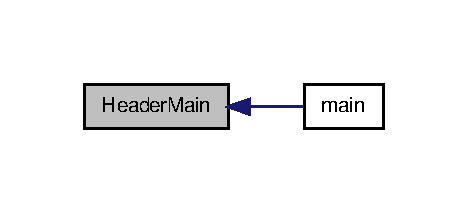
\includegraphics[width=224pt]{_bradshaw-_mansfield-_assn2-_h_a_s_h_prog_8cpp_ad0ff1b56e8aa2267183dc975be2704c3_icgraph}
\end{center}
\end{figure}


\hypertarget{_bradshaw-_mansfield-_assn2-_h_a_s_h_prog_8cpp_a74bb3e2823ba913f28e3f6711e045824}{
\index{Bradshaw-\/Mansfield-\/Assn2-\/HASHProg.cpp@{Bradshaw-\/Mansfield-\/Assn2-\/HASHProg.cpp}!LinearProbe@{LinearProbe}}
\index{LinearProbe@{LinearProbe}!Bradshaw-Mansfield-Assn2-HASHProg.cpp@{Bradshaw-\/Mansfield-\/Assn2-\/HASHProg.cpp}}
\subsubsection[{LinearProbe}]{\setlength{\rightskip}{0pt plus 5cm}void LinearProbe (
\begin{DoxyParamCaption}
\item[{int \&}]{address, }
\item[{int}]{hashTable\mbox{[}$\,$\mbox{]}, }
\item[{int}]{probeThis, }
\item[{int}]{tbSize, }
\item[{int \&}]{colCount}
\end{DoxyParamCaption}
)}}
\label{_bradshaw-_mansfield-_assn2-_h_a_s_h_prog_8cpp_a74bb3e2823ba913f28e3f6711e045824}
FUNCTION: LinearProbe DESCRIPTION: Incrementally checks each and every index for available empty memory in array. Keeps counter of number of attempts before valid enry is found. INPUT: Parameters: address: Current address hashTable: Array being used probeThis: Int being searched for 0 if looking for empty index htSize: Hash Table size colCount: The count of how many searches were performed. OUTPUT: Parameters: address: Address of valid location colCount: The count of how many searches were performed. IMPLEMENTED BY: Jason Mansfield 

Definition at line 422 of file Bradshaw-\/Mansfield-\/Assn2-\/HASHProg.cpp.



Here is the caller graph for this function:\nopagebreak
\begin{figure}[H]
\begin{center}
\leavevmode
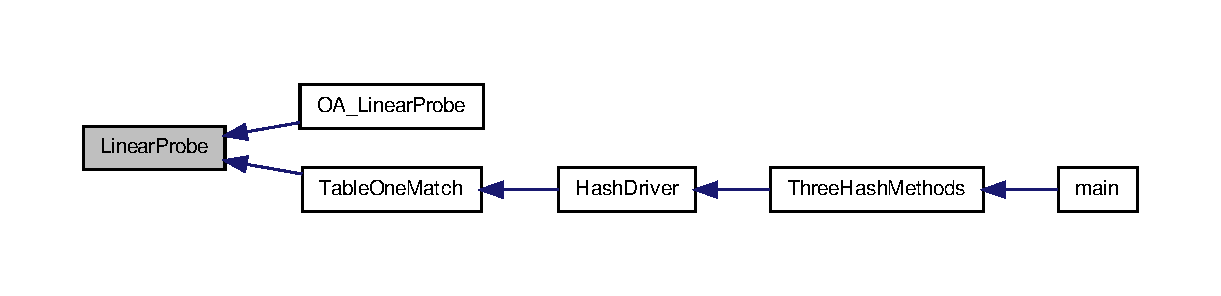
\includegraphics[width=400pt]{_bradshaw-_mansfield-_assn2-_h_a_s_h_prog_8cpp_a74bb3e2823ba913f28e3f6711e045824_icgraph}
\end{center}
\end{figure}


\hypertarget{_bradshaw-_mansfield-_assn2-_h_a_s_h_prog_8cpp_ae66f6b31b5ad750f1fe042a706a4e3d4}{
\index{Bradshaw-\/Mansfield-\/Assn2-\/HASHProg.cpp@{Bradshaw-\/Mansfield-\/Assn2-\/HASHProg.cpp}!main@{main}}
\index{main@{main}!Bradshaw-Mansfield-Assn2-HASHProg.cpp@{Bradshaw-\/Mansfield-\/Assn2-\/HASHProg.cpp}}
\subsubsection[{main}]{\setlength{\rightskip}{0pt plus 5cm}int main (
\begin{DoxyParamCaption}
{}
\end{DoxyParamCaption}
)}}
\label{_bradshaw-_mansfield-_assn2-_h_a_s_h_prog_8cpp_ae66f6b31b5ad750f1fe042a706a4e3d4}
FUNCTION: \hyperlink{_bradshaw-_mansfield-_assn2-_h_a_s_h_prog_8cpp_ae66f6b31b5ad750f1fe042a706a4e3d4}{main()} DESCRIPTION: simple main function OUTPUT: Return Val: returns 0 if success CALLS TO: \hyperlink{_bradshaw-_mansfield-_assn2-_h_a_s_h_prog_8cpp_ac4885dc21b261220f2a030b1ad06aec5}{ThreeHashMethods()} IMPLEMENTED BY: Jeremy and Jason 

Definition at line 92 of file Bradshaw-\/Mansfield-\/Assn2-\/HASHProg.cpp.



Here is the call graph for this function:\nopagebreak
\begin{figure}[H]
\begin{center}
\leavevmode
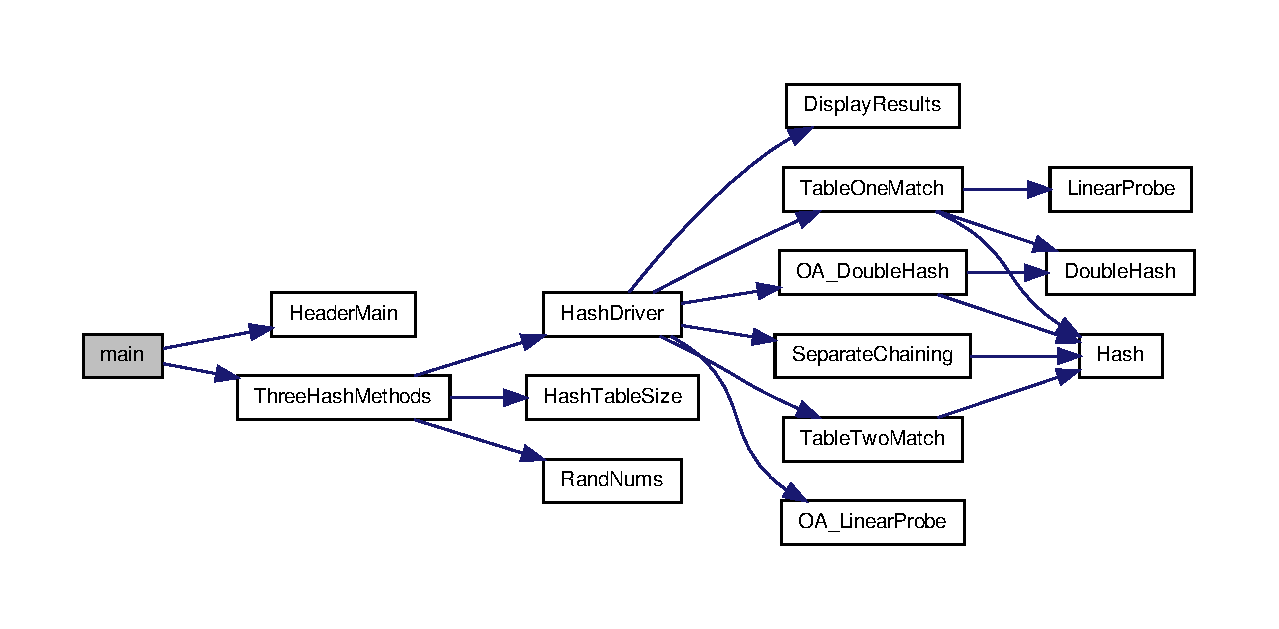
\includegraphics[width=400pt]{_bradshaw-_mansfield-_assn2-_h_a_s_h_prog_8cpp_ae66f6b31b5ad750f1fe042a706a4e3d4_cgraph}
\end{center}
\end{figure}


\hypertarget{_bradshaw-_mansfield-_assn2-_h_a_s_h_prog_8cpp_aa08a3d5e09643b1011e506d60a89a7f2}{
\index{Bradshaw-\/Mansfield-\/Assn2-\/HASHProg.cpp@{Bradshaw-\/Mansfield-\/Assn2-\/HASHProg.cpp}!OA\_\-DoubleHash@{OA\_\-DoubleHash}}
\index{OA\_\-DoubleHash@{OA\_\-DoubleHash}!Bradshaw-Mansfield-Assn2-HASHProg.cpp@{Bradshaw-\/Mansfield-\/Assn2-\/HASHProg.cpp}}
\subsubsection[{OA\_\-DoubleHash}]{\setlength{\rightskip}{0pt plus 5cm}void OA\_\-DoubleHash (
\begin{DoxyParamCaption}
\item[{int $\ast$}]{randArray, }
\item[{int}]{tbSize, }
\item[{int}]{hashTable\mbox{[}$\,$\mbox{]}, }
\item[{bool \&}]{infiniteLoop}
\end{DoxyParamCaption}
)}}
\label{_bradshaw-_mansfield-_assn2-_h_a_s_h_prog_8cpp_aa08a3d5e09643b1011e506d60a89a7f2}
FUNCTION: OA\_\-DoubleHash DESCRIPTION: Open Addressing with use of DoubleHash INPUT: Parameters: $\ast$randArray: array of random int tbSize: requested hash table size hasTable: empty array for hash table OUTPUT: Parameters: hashTable: hash table with hashed data from random array. infiniteLoop: Bool test for an infinite loop error CALLS TO: \hyperlink{_bradshaw-_mansfield-_assn2-_h_a_s_h_prog_8cpp_a7b947e56197fe93937e40b0c987f40fb}{DoubleHash()} \hyperlink{_bradshaw-_mansfield-_assn2-_h_a_s_h_prog_8cpp_ae9957e8e2a204d621e9f9cc2999adf56}{Hash()} IMPLEMENTED BY: Jeremy Bradshaw 

Definition at line 495 of file Bradshaw-\/Mansfield-\/Assn2-\/HASHProg.cpp.



Here is the call graph for this function:\nopagebreak
\begin{figure}[H]
\begin{center}
\leavevmode
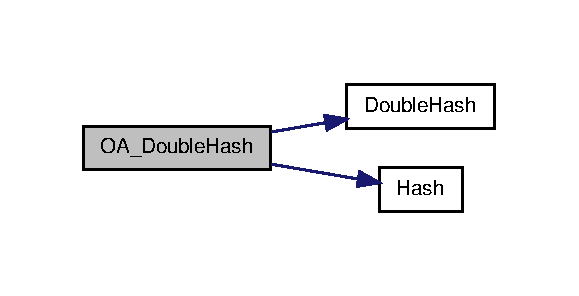
\includegraphics[width=278pt]{_bradshaw-_mansfield-_assn2-_h_a_s_h_prog_8cpp_aa08a3d5e09643b1011e506d60a89a7f2_cgraph}
\end{center}
\end{figure}




Here is the caller graph for this function:\nopagebreak
\begin{figure}[H]
\begin{center}
\leavevmode
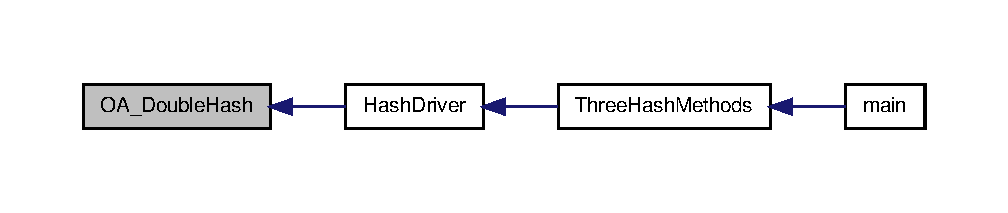
\includegraphics[width=400pt]{_bradshaw-_mansfield-_assn2-_h_a_s_h_prog_8cpp_aa08a3d5e09643b1011e506d60a89a7f2_icgraph}
\end{center}
\end{figure}


\hypertarget{_bradshaw-_mansfield-_assn2-_h_a_s_h_prog_8cpp_aa342d426f7a6fa643a100ba04bc8e46e}{
\index{Bradshaw-\/Mansfield-\/Assn2-\/HASHProg.cpp@{Bradshaw-\/Mansfield-\/Assn2-\/HASHProg.cpp}!OA\_\-LinearProbe@{OA\_\-LinearProbe}}
\index{OA\_\-LinearProbe@{OA\_\-LinearProbe}!Bradshaw-Mansfield-Assn2-HASHProg.cpp@{Bradshaw-\/Mansfield-\/Assn2-\/HASHProg.cpp}}
\subsubsection[{OA\_\-LinearProbe}]{\setlength{\rightskip}{0pt plus 5cm}int$\ast$ OA\_\-LinearProbe (
\begin{DoxyParamCaption}
\item[{int $\ast$}]{randArray, }
\item[{int}]{tbSize, }
\item[{int $\ast$}]{hashTable}
\end{DoxyParamCaption}
)}}
\label{_bradshaw-_mansfield-_assn2-_h_a_s_h_prog_8cpp_aa342d426f7a6fa643a100ba04bc8e46e}
FUNCTION: OA\_\-LinearProbe DESCRIPTION: Open Addressing with use of Linear Probe INPUT: Parameters: $\ast$randArray: Array of random int tbSize: Requested hash table size hashTable: Empty array for hash table OUTPUT: Return Val: hashTable: Hash table with hashed data from random array. CALLS TO: \hyperlink{_bradshaw-_mansfield-_assn2-_h_a_s_h_prog_8cpp_a74bb3e2823ba913f28e3f6711e045824}{LinearProbe()} \hyperlink{_bradshaw-_mansfield-_assn2-_h_a_s_h_prog_8cpp_ae9957e8e2a204d621e9f9cc2999adf56}{Hash()} IMPLEMENTED BY: Jason Mansfield 

Definition at line 383 of file Bradshaw-\/Mansfield-\/Assn2-\/HASHProg.cpp.



Here is the call graph for this function:\nopagebreak
\begin{figure}[H]
\begin{center}
\leavevmode
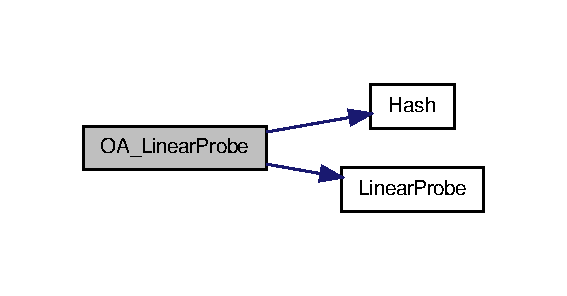
\includegraphics[width=272pt]{_bradshaw-_mansfield-_assn2-_h_a_s_h_prog_8cpp_aa342d426f7a6fa643a100ba04bc8e46e_cgraph}
\end{center}
\end{figure}


\hypertarget{_bradshaw-_mansfield-_assn2-_h_a_s_h_prog_8cpp_aa4c8e3922c8cd75082eae40ba8cd0205}{
\index{Bradshaw-\/Mansfield-\/Assn2-\/HASHProg.cpp@{Bradshaw-\/Mansfield-\/Assn2-\/HASHProg.cpp}!OA\_\-LinearProbe@{OA\_\-LinearProbe}}
\index{OA\_\-LinearProbe@{OA\_\-LinearProbe}!Bradshaw-Mansfield-Assn2-HASHProg.cpp@{Bradshaw-\/Mansfield-\/Assn2-\/HASHProg.cpp}}
\subsubsection[{OA\_\-LinearProbe}]{\setlength{\rightskip}{0pt plus 5cm}int$\ast$ OA\_\-LinearProbe (
\begin{DoxyParamCaption}
\item[{int $\ast$}]{, }
\item[{int}]{, }
\item[{int}]{\mbox{[}$\,$\mbox{]}}
\end{DoxyParamCaption}
)}}
\label{_bradshaw-_mansfield-_assn2-_h_a_s_h_prog_8cpp_aa4c8e3922c8cd75082eae40ba8cd0205}


Here is the caller graph for this function:\nopagebreak
\begin{figure}[H]
\begin{center}
\leavevmode
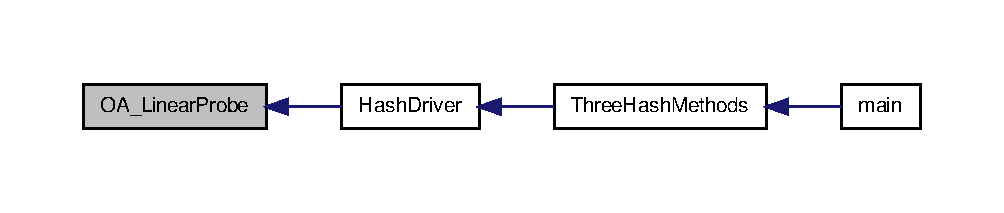
\includegraphics[width=400pt]{_bradshaw-_mansfield-_assn2-_h_a_s_h_prog_8cpp_aa4c8e3922c8cd75082eae40ba8cd0205_icgraph}
\end{center}
\end{figure}


\hypertarget{_bradshaw-_mansfield-_assn2-_h_a_s_h_prog_8cpp_ad02a3d3bea24e6a374d52753e741ae54}{
\index{Bradshaw-\/Mansfield-\/Assn2-\/HASHProg.cpp@{Bradshaw-\/Mansfield-\/Assn2-\/HASHProg.cpp}!RandNums@{RandNums}}
\index{RandNums@{RandNums}!Bradshaw-Mansfield-Assn2-HASHProg.cpp@{Bradshaw-\/Mansfield-\/Assn2-\/HASHProg.cpp}}
\subsubsection[{RandNums}]{\setlength{\rightskip}{0pt plus 5cm}int RandNums (
\begin{DoxyParamCaption}
\item[{int $\ast$}]{randArray}
\end{DoxyParamCaption}
)}}
\label{_bradshaw-_mansfield-_assn2-_h_a_s_h_prog_8cpp_ad02a3d3bea24e6a374d52753e741ae54}
FUNCTION: \hyperlink{_bradshaw-_mansfield-_assn2-_h_a_s_h_prog_8cpp_ad02a3d3bea24e6a374d52753e741ae54}{RandNums()} DESCRIPTION: Creates array of MAX\_\-KEYS amount of random numbers INPUT: Parameters: $\ast$randArray: Empty array OUTPUT: Return Val: $\ast$randArray: with MAX\_\-KEYS amount of random ints. IMPLEMENTED BY: Jason Mansfield 

Definition at line 167 of file Bradshaw-\/Mansfield-\/Assn2-\/HASHProg.cpp.



Here is the caller graph for this function:\nopagebreak
\begin{figure}[H]
\begin{center}
\leavevmode
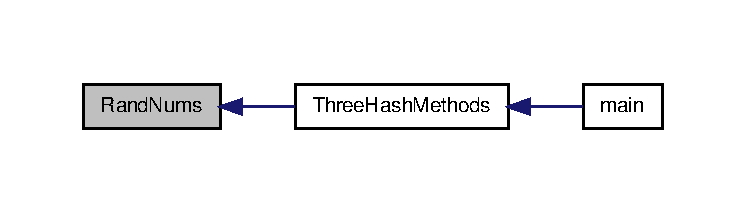
\includegraphics[width=358pt]{_bradshaw-_mansfield-_assn2-_h_a_s_h_prog_8cpp_ad02a3d3bea24e6a374d52753e741ae54_icgraph}
\end{center}
\end{figure}


\hypertarget{_bradshaw-_mansfield-_assn2-_h_a_s_h_prog_8cpp_ad730cee6dc4ea13d5fabcec47b736c79}{
\index{Bradshaw-\/Mansfield-\/Assn2-\/HASHProg.cpp@{Bradshaw-\/Mansfield-\/Assn2-\/HASHProg.cpp}!SeparateChaining@{SeparateChaining}}
\index{SeparateChaining@{SeparateChaining}!Bradshaw-Mansfield-Assn2-HASHProg.cpp@{Bradshaw-\/Mansfield-\/Assn2-\/HASHProg.cpp}}
\subsubsection[{SeparateChaining}]{\setlength{\rightskip}{0pt plus 5cm}void SeparateChaining (
\begin{DoxyParamCaption}
\item[{int $\ast$}]{randArray, }
\item[{int}]{tbSize, }
\item[{{\bf TABLE}}]{chainingArray\mbox{[}$\,$\mbox{]}}
\end{DoxyParamCaption}
)}}
\label{_bradshaw-_mansfield-_assn2-_h_a_s_h_prog_8cpp_ad730cee6dc4ea13d5fabcec47b736c79}
FUNCTION: SeparateChaining DESCRIPTION: Uses seperate chaining to create single linked lists of data. Linked list is used for collisions. INPUT: Parameters: $\ast$randArray: Array of random int tbSize: Requested hash table size chainingArray: Empty array of struct \hyperlink{struct_t_a_b_l_e}{TABLE} for linked list. OUTPUT: Parameters: $\ast$chainingArray : becomes an array of linked list data containing random array int. CALLS TO: \hyperlink{_bradshaw-_mansfield-_assn2-_h_a_s_h_prog_8cpp_ae9957e8e2a204d621e9f9cc2999adf56}{Hash()} IMPLEMENTED BY: Jeremy Bradshaw 

Definition at line 541 of file Bradshaw-\/Mansfield-\/Assn2-\/HASHProg.cpp.



Here is the call graph for this function:\nopagebreak
\begin{figure}[H]
\begin{center}
\leavevmode
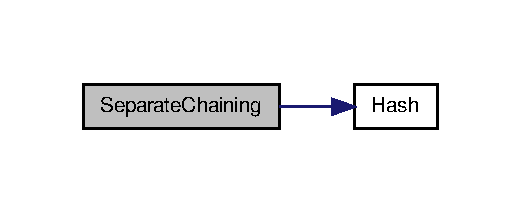
\includegraphics[width=250pt]{_bradshaw-_mansfield-_assn2-_h_a_s_h_prog_8cpp_ad730cee6dc4ea13d5fabcec47b736c79_cgraph}
\end{center}
\end{figure}




Here is the caller graph for this function:\nopagebreak
\begin{figure}[H]
\begin{center}
\leavevmode
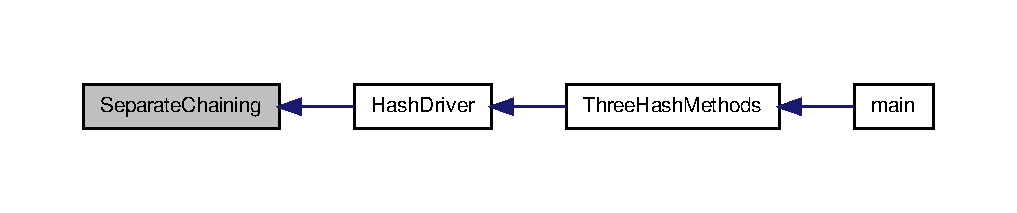
\includegraphics[width=400pt]{_bradshaw-_mansfield-_assn2-_h_a_s_h_prog_8cpp_ad730cee6dc4ea13d5fabcec47b736c79_icgraph}
\end{center}
\end{figure}


\hypertarget{_bradshaw-_mansfield-_assn2-_h_a_s_h_prog_8cpp_a1cfe5833c4e03ff0473ca3e3b87f9f1d}{
\index{Bradshaw-\/Mansfield-\/Assn2-\/HASHProg.cpp@{Bradshaw-\/Mansfield-\/Assn2-\/HASHProg.cpp}!TableOneMatch@{TableOneMatch}}
\index{TableOneMatch@{TableOneMatch}!Bradshaw-Mansfield-Assn2-HASHProg.cpp@{Bradshaw-\/Mansfield-\/Assn2-\/HASHProg.cpp}}
\subsubsection[{TableOneMatch}]{\setlength{\rightskip}{0pt plus 5cm}int TableOneMatch (
\begin{DoxyParamCaption}
\item[{int $\ast$}]{randArray, }
\item[{int $\ast$}]{ht, }
\item[{int}]{tbSize, }
\item[{int}]{loop, }
\item[{int}]{colCount}
\end{DoxyParamCaption}
)}}
\label{_bradshaw-_mansfield-_assn2-_h_a_s_h_prog_8cpp_a1cfe5833c4e03ff0473ca3e3b87f9f1d}
FUNCTION: TableOneMatch DESCRIPTION: Matches original random array data against newly created ht hash table. INPUT: Parameters: randArray: Original random array of int used to load hash table ht: Freshly created hash table containing random array tbSize: Hash table size loop: Assists HashDriver function with reuse of TableOneMatch -\/0 allows call to LinearProbe on first call -\/1 allows call to DoubleHash on second call OUTPUT: Return Value: colCount: The count of how many searches were performed. CALLS TO: \hyperlink{_bradshaw-_mansfield-_assn2-_h_a_s_h_prog_8cpp_a74bb3e2823ba913f28e3f6711e045824}{LinearProbe()} \hyperlink{_bradshaw-_mansfield-_assn2-_h_a_s_h_prog_8cpp_a7b947e56197fe93937e40b0c987f40fb}{DoubleHash()} \hyperlink{_bradshaw-_mansfield-_assn2-_h_a_s_h_prog_8cpp_ae9957e8e2a204d621e9f9cc2999adf56}{Hash()} IMPLEMENTED BY: Jason Mansfield 

Definition at line 597 of file Bradshaw-\/Mansfield-\/Assn2-\/HASHProg.cpp.



Here is the call graph for this function:\nopagebreak
\begin{figure}[H]
\begin{center}
\leavevmode
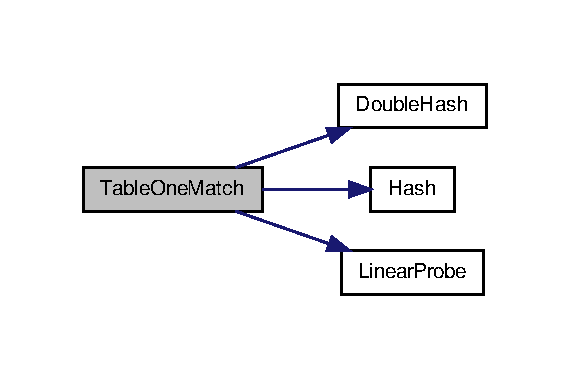
\includegraphics[width=274pt]{_bradshaw-_mansfield-_assn2-_h_a_s_h_prog_8cpp_a1cfe5833c4e03ff0473ca3e3b87f9f1d_cgraph}
\end{center}
\end{figure}




Here is the caller graph for this function:\nopagebreak
\begin{figure}[H]
\begin{center}
\leavevmode
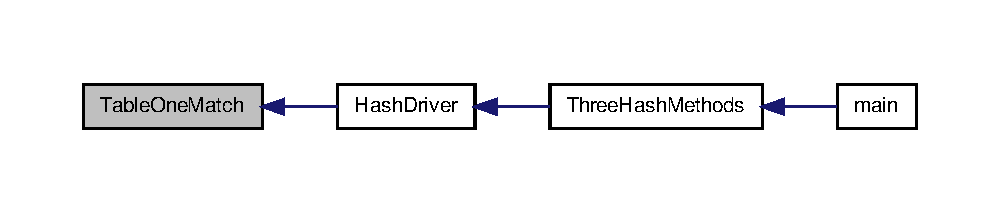
\includegraphics[width=400pt]{_bradshaw-_mansfield-_assn2-_h_a_s_h_prog_8cpp_a1cfe5833c4e03ff0473ca3e3b87f9f1d_icgraph}
\end{center}
\end{figure}


\hypertarget{_bradshaw-_mansfield-_assn2-_h_a_s_h_prog_8cpp_ab7be41246bbc3491cbe4151458a15f39}{
\index{Bradshaw-\/Mansfield-\/Assn2-\/HASHProg.cpp@{Bradshaw-\/Mansfield-\/Assn2-\/HASHProg.cpp}!TableTwoMatch@{TableTwoMatch}}
\index{TableTwoMatch@{TableTwoMatch}!Bradshaw-Mansfield-Assn2-HASHProg.cpp@{Bradshaw-\/Mansfield-\/Assn2-\/HASHProg.cpp}}
\subsubsection[{TableTwoMatch}]{\setlength{\rightskip}{0pt plus 5cm}int TableTwoMatch (
\begin{DoxyParamCaption}
\item[{int $\ast$}]{randArray, }
\item[{{\bf TABLE}}]{chainingArray\mbox{[}$\,$\mbox{]}, }
\item[{int}]{colCount, }
\item[{int}]{tbSize}
\end{DoxyParamCaption}
)}}
\label{_bradshaw-_mansfield-_assn2-_h_a_s_h_prog_8cpp_ab7be41246bbc3491cbe4151458a15f39}
FUNCTION: TableTwoMatch DESCRIPTION: Traverses and matches original random array with freshly created inked list of random data. INPUT: Parameters: $\ast$randArray: Original random array used to make hashed linked list chainingArray: Linked list containing hashed data OUTPUT: ReturnValue: colCount: The count of how many searches were performed.

CALLS TO: HASH() IMPLEMENTED BY: Jeremy Bradshaw 

Definition at line 662 of file Bradshaw-\/Mansfield-\/Assn2-\/HASHProg.cpp.



Here is the call graph for this function:\nopagebreak
\begin{figure}[H]
\begin{center}
\leavevmode
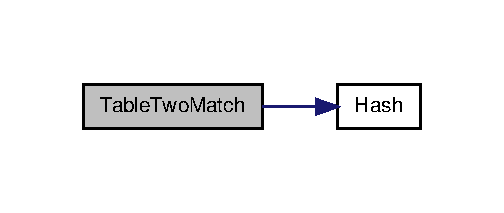
\includegraphics[width=242pt]{_bradshaw-_mansfield-_assn2-_h_a_s_h_prog_8cpp_ab7be41246bbc3491cbe4151458a15f39_cgraph}
\end{center}
\end{figure}




Here is the caller graph for this function:\nopagebreak
\begin{figure}[H]
\begin{center}
\leavevmode
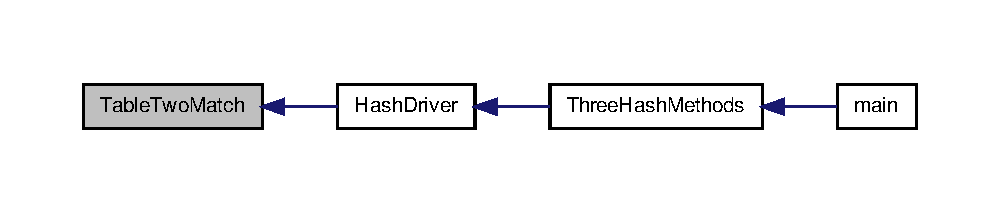
\includegraphics[width=400pt]{_bradshaw-_mansfield-_assn2-_h_a_s_h_prog_8cpp_ab7be41246bbc3491cbe4151458a15f39_icgraph}
\end{center}
\end{figure}


\hypertarget{_bradshaw-_mansfield-_assn2-_h_a_s_h_prog_8cpp_ac4885dc21b261220f2a030b1ad06aec5}{
\index{Bradshaw-\/Mansfield-\/Assn2-\/HASHProg.cpp@{Bradshaw-\/Mansfield-\/Assn2-\/HASHProg.cpp}!ThreeHashMethods@{ThreeHashMethods}}
\index{ThreeHashMethods@{ThreeHashMethods}!Bradshaw-Mansfield-Assn2-HASHProg.cpp@{Bradshaw-\/Mansfield-\/Assn2-\/HASHProg.cpp}}
\subsubsection[{ThreeHashMethods}]{\setlength{\rightskip}{0pt plus 5cm}void ThreeHashMethods (
\begin{DoxyParamCaption}
{}
\end{DoxyParamCaption}
)}}
\label{_bradshaw-_mansfield-_assn2-_h_a_s_h_prog_8cpp_ac4885dc21b261220f2a030b1ad06aec5}
FUNCTION: \hyperlink{_bradshaw-_mansfield-_assn2-_h_a_s_h_prog_8cpp_ac4885dc21b261220f2a030b1ad06aec5}{ThreeHashMethods()} DESCRIPTION: Calls functions to load randArray numbers, prompt user hash table size, and calls HashDriver. Displays data regarding the load factor, MAX\_\-KEYS and tbSize CALLS TO: \hyperlink{_bradshaw-_mansfield-_assn2-_h_a_s_h_prog_8cpp_ad02a3d3bea24e6a374d52753e741ae54}{RandNums()} \hyperlink{_bradshaw-_mansfield-_assn2-_h_a_s_h_prog_8cpp_a0ab6301502b50757d27084788bab0db3}{HashTableSize()} \hyperlink{_bradshaw-_mansfield-_assn2-_h_a_s_h_prog_8cpp_acb3d9aabc9ab7fbb9d3ae15ad62c32f1}{HashDriver()}. IMPLEMENTED BY: Jason Mansfield 

Definition at line 242 of file Bradshaw-\/Mansfield-\/Assn2-\/HASHProg.cpp.



Here is the call graph for this function:\nopagebreak
\begin{figure}[H]
\begin{center}
\leavevmode
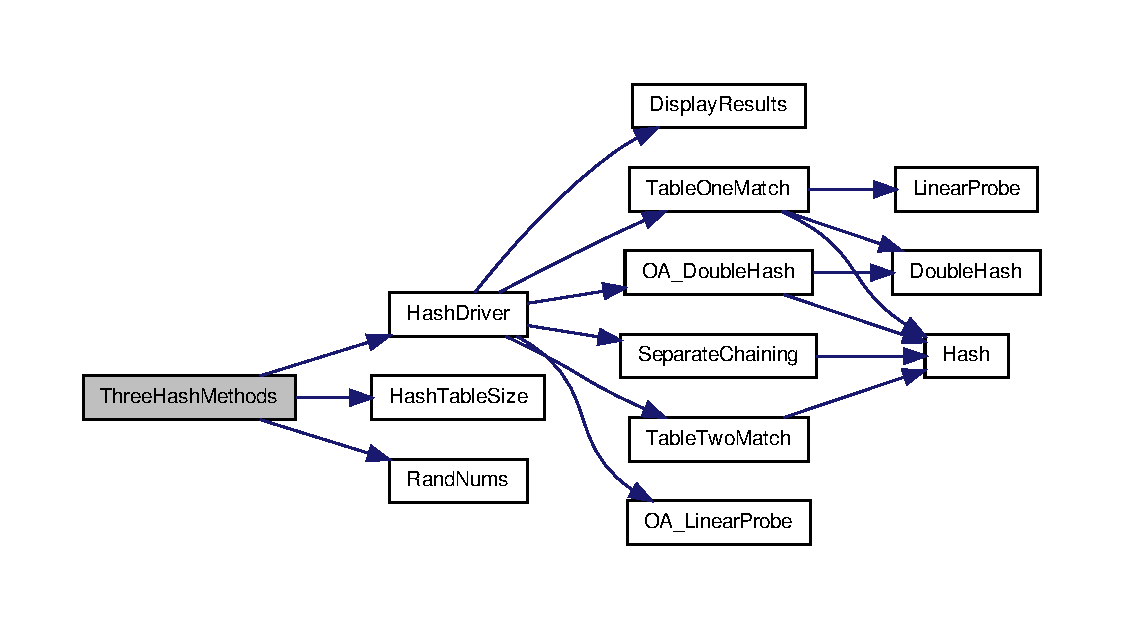
\includegraphics[width=400pt]{_bradshaw-_mansfield-_assn2-_h_a_s_h_prog_8cpp_ac4885dc21b261220f2a030b1ad06aec5_cgraph}
\end{center}
\end{figure}




Here is the caller graph for this function:\nopagebreak
\begin{figure}[H]
\begin{center}
\leavevmode
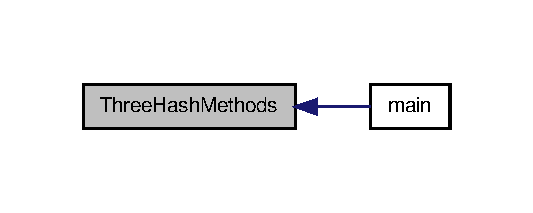
\includegraphics[width=256pt]{_bradshaw-_mansfield-_assn2-_h_a_s_h_prog_8cpp_ac4885dc21b261220f2a030b1ad06aec5_icgraph}
\end{center}
\end{figure}




\subsection{Variable Documentation}
\hypertarget{_bradshaw-_mansfield-_assn2-_h_a_s_h_prog_8cpp_a80697a51c12117a5eae4ada58d27e1c2}{
\index{Bradshaw-\/Mansfield-\/Assn2-\/HASHProg.cpp@{Bradshaw-\/Mansfield-\/Assn2-\/HASHProg.cpp}!MAX\_\-INT\_\-SIZE@{MAX\_\-INT\_\-SIZE}}
\index{MAX\_\-INT\_\-SIZE@{MAX\_\-INT\_\-SIZE}!Bradshaw-Mansfield-Assn2-HASHProg.cpp@{Bradshaw-\/Mansfield-\/Assn2-\/HASHProg.cpp}}
\subsubsection[{MAX\_\-INT\_\-SIZE}]{\setlength{\rightskip}{0pt plus 5cm}const int {\bf MAX\_\-INT\_\-SIZE} = 30000}}
\label{_bradshaw-_mansfield-_assn2-_h_a_s_h_prog_8cpp_a80697a51c12117a5eae4ada58d27e1c2}


Definition at line 53 of file Bradshaw-\/Mansfield-\/Assn2-\/HASHProg.cpp.

\hypertarget{_bradshaw-_mansfield-_assn2-_h_a_s_h_prog_8cpp_ad2624222b2a41e40f795baff70c1d20c}{
\index{Bradshaw-\/Mansfield-\/Assn2-\/HASHProg.cpp@{Bradshaw-\/Mansfield-\/Assn2-\/HASHProg.cpp}!MAX\_\-KEYS@{MAX\_\-KEYS}}
\index{MAX\_\-KEYS@{MAX\_\-KEYS}!Bradshaw-Mansfield-Assn2-HASHProg.cpp@{Bradshaw-\/Mansfield-\/Assn2-\/HASHProg.cpp}}
\subsubsection[{MAX\_\-KEYS}]{\setlength{\rightskip}{0pt plus 5cm}const int {\bf MAX\_\-KEYS} = 5000}}
\label{_bradshaw-_mansfield-_assn2-_h_a_s_h_prog_8cpp_ad2624222b2a41e40f795baff70c1d20c}


Definition at line 57 of file Bradshaw-\/Mansfield-\/Assn2-\/HASHProg.cpp.

\hypertarget{_bradshaw-_mansfield-_assn2-_h_a_s_h_prog_8cpp_a3a0ca86f28ff2c4d31143f5f3d6ca40a}{
\index{Bradshaw-\/Mansfield-\/Assn2-\/HASHProg.cpp@{Bradshaw-\/Mansfield-\/Assn2-\/HASHProg.cpp}!MAX\_\-KEYS\_\-DBL@{MAX\_\-KEYS\_\-DBL}}
\index{MAX\_\-KEYS\_\-DBL@{MAX\_\-KEYS\_\-DBL}!Bradshaw-Mansfield-Assn2-HASHProg.cpp@{Bradshaw-\/Mansfield-\/Assn2-\/HASHProg.cpp}}
\subsubsection[{MAX\_\-KEYS\_\-DBL}]{\setlength{\rightskip}{0pt plus 5cm}const double {\bf MAX\_\-KEYS\_\-DBL} = 5000.00}}
\label{_bradshaw-_mansfield-_assn2-_h_a_s_h_prog_8cpp_a3a0ca86f28ff2c4d31143f5f3d6ca40a}


Definition at line 60 of file Bradshaw-\/Mansfield-\/Assn2-\/HASHProg.cpp.

\hypertarget{_bradshaw-_mansfield-_assn2-_h_a_s_h_prog_8cpp_a92e00f871716652e494af2741a4794bd}{
\index{Bradshaw-\/Mansfield-\/Assn2-\/HASHProg.cpp@{Bradshaw-\/Mansfield-\/Assn2-\/HASHProg.cpp}!MIN\_\-HASH\_\-TABLE\_\-SIZE@{MIN\_\-HASH\_\-TABLE\_\-SIZE}}
\index{MIN\_\-HASH\_\-TABLE\_\-SIZE@{MIN\_\-HASH\_\-TABLE\_\-SIZE}!Bradshaw-Mansfield-Assn2-HASHProg.cpp@{Bradshaw-\/Mansfield-\/Assn2-\/HASHProg.cpp}}
\subsubsection[{MIN\_\-HASH\_\-TABLE\_\-SIZE}]{\setlength{\rightskip}{0pt plus 5cm}const int {\bf MIN\_\-HASH\_\-TABLE\_\-SIZE} = 6500}}
\label{_bradshaw-_mansfield-_assn2-_h_a_s_h_prog_8cpp_a92e00f871716652e494af2741a4794bd}


Definition at line 56 of file Bradshaw-\/Mansfield-\/Assn2-\/HASHProg.cpp.

\hypertarget{_bradshaw-_mansfield-_assn2-_h_a_s_h_prog_8cpp_a2e30ee6cd6a71066a4c99da7204c73bd}{
\index{Bradshaw-\/Mansfield-\/Assn2-\/HASHProg.cpp@{Bradshaw-\/Mansfield-\/Assn2-\/HASHProg.cpp}!MIN\_\-INT\_\-SIZE@{MIN\_\-INT\_\-SIZE}}
\index{MIN\_\-INT\_\-SIZE@{MIN\_\-INT\_\-SIZE}!Bradshaw-Mansfield-Assn2-HASHProg.cpp@{Bradshaw-\/Mansfield-\/Assn2-\/HASHProg.cpp}}
\subsubsection[{MIN\_\-INT\_\-SIZE}]{\setlength{\rightskip}{0pt plus 5cm}const int {\bf MIN\_\-INT\_\-SIZE} = 1}}
\label{_bradshaw-_mansfield-_assn2-_h_a_s_h_prog_8cpp_a2e30ee6cd6a71066a4c99da7204c73bd}


Definition at line 54 of file Bradshaw-\/Mansfield-\/Assn2-\/HASHProg.cpp.

\hypertarget{_bradshaw-_mansfield-_assn2-_h_a_s_h_prog_8cpp_a02ce5f32cab205c8455bd8b976085c50}{
\index{Bradshaw-\/Mansfield-\/Assn2-\/HASHProg.cpp@{Bradshaw-\/Mansfield-\/Assn2-\/HASHProg.cpp}!NUM\_\-ITEMS\_\-TO\_\-SEARCH@{NUM\_\-ITEMS\_\-TO\_\-SEARCH}}
\index{NUM\_\-ITEMS\_\-TO\_\-SEARCH@{NUM\_\-ITEMS\_\-TO\_\-SEARCH}!Bradshaw-Mansfield-Assn2-HASHProg.cpp@{Bradshaw-\/Mansfield-\/Assn2-\/HASHProg.cpp}}
\subsubsection[{NUM\_\-ITEMS\_\-TO\_\-SEARCH}]{\setlength{\rightskip}{0pt plus 5cm}const int {\bf NUM\_\-ITEMS\_\-TO\_\-SEARCH} = 2500}}
\label{_bradshaw-_mansfield-_assn2-_h_a_s_h_prog_8cpp_a02ce5f32cab205c8455bd8b976085c50}


Definition at line 58 of file Bradshaw-\/Mansfield-\/Assn2-\/HASHProg.cpp.

\hypertarget{_bradshaw-_mansfield-_assn2-_h_a_s_h_prog_8cpp_ad619de5a53a38d732b9c5da01523a23e}{
\index{Bradshaw-\/Mansfield-\/Assn2-\/HASHProg.cpp@{Bradshaw-\/Mansfield-\/Assn2-\/HASHProg.cpp}!NUM\_\-ITEMS\_\-TO\_\-SEARCH\_\-DBL@{NUM\_\-ITEMS\_\-TO\_\-SEARCH\_\-DBL}}
\index{NUM\_\-ITEMS\_\-TO\_\-SEARCH\_\-DBL@{NUM\_\-ITEMS\_\-TO\_\-SEARCH\_\-DBL}!Bradshaw-Mansfield-Assn2-HASHProg.cpp@{Bradshaw-\/Mansfield-\/Assn2-\/HASHProg.cpp}}
\subsubsection[{NUM\_\-ITEMS\_\-TO\_\-SEARCH\_\-DBL}]{\setlength{\rightskip}{0pt plus 5cm}const double {\bf NUM\_\-ITEMS\_\-TO\_\-SEARCH\_\-DBL} = 2500.00}}
\label{_bradshaw-_mansfield-_assn2-_h_a_s_h_prog_8cpp_ad619de5a53a38d732b9c5da01523a23e}


Definition at line 59 of file Bradshaw-\/Mansfield-\/Assn2-\/HASHProg.cpp.

\hypertarget{_bradshaw-_mansfield-_assn2-_h_a_s_h_prog_8cpp_ac3e309d0e80c3dd569ed3cfb701075a8}{
\index{Bradshaw-\/Mansfield-\/Assn2-\/HASHProg.cpp@{Bradshaw-\/Mansfield-\/Assn2-\/HASHProg.cpp}!NUM\_\-PROBING\_\-LOOPS@{NUM\_\-PROBING\_\-LOOPS}}
\index{NUM\_\-PROBING\_\-LOOPS@{NUM\_\-PROBING\_\-LOOPS}!Bradshaw-Mansfield-Assn2-HASHProg.cpp@{Bradshaw-\/Mansfield-\/Assn2-\/HASHProg.cpp}}
\subsubsection[{NUM\_\-PROBING\_\-LOOPS}]{\setlength{\rightskip}{0pt plus 5cm}const int {\bf NUM\_\-PROBING\_\-LOOPS} = 3}}
\label{_bradshaw-_mansfield-_assn2-_h_a_s_h_prog_8cpp_ac3e309d0e80c3dd569ed3cfb701075a8}


Definition at line 55 of file Bradshaw-\/Mansfield-\/Assn2-\/HASHProg.cpp.


\printindex
\end{document}
